% Chapter 1

\chapter{Einführung} % Chapter title

\label{ch:introduction} % For referencing the chapter elsewhere, use \autoref{ch:introduction} 

%----------------------------------------------------------------------------------------

\section{Geschichte der Kryptographie}

%---------

\paragraph{Altertum}
\hfill\\
Erste frühe Varianten waren geheimnachrichten die versteckt Transportiert wurden.\\
So wurden beispielweise in Ägypten Sklaven die Haare abrasiert eine Nachricht eintätowiert und nachdem die Haara nachgewachsen waren zum Empfänger geschickt.
Eine weitere Variante waren kleine Löcher in Buchstabenform auf Papyrusrollen, die erst bei Gegenlicht dann sichtbar wurden.
\\ Auch in Griechenland wurde bereits 500 v.Chr. ein Verschlüsselungsstab namens Skytale\footnote{\url{https://de.wikipedia.org/wiki/Skytale}} Entwickelt mit deren Hilfe Texte verschlüsselt werden konnten.

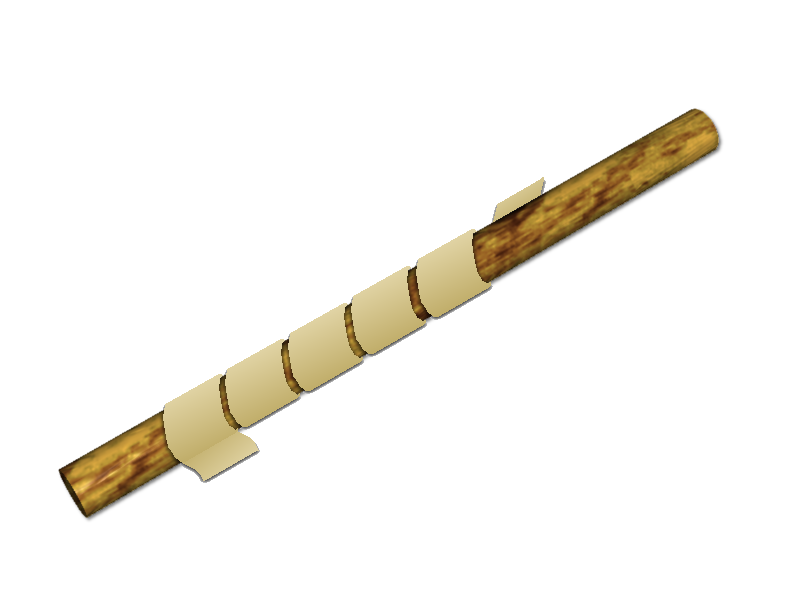
\includegraphics[width=5cm]{gfx/Skytala}% Picture
\hfill
\\ Julius Cäsar (etwa 100 v. Chr. bis 44 v. Chr.) soll die nach ihm benannte Cäsar-Chiffre \footnote{\url{https://de.wikipedia.org/wiki/Gaius_Iulius_Caesar}} genutzt haben, die jeden Buchstaben im Alphabet um einen festgelegten Wert verschiebt.

%---------

\paragraph{Mittelalter}
\hfill\\
\citeauthor{al-kadi}Zwischen den Jahren 500 und 1400 gab es vor allem aus der arabischen Welt bedeutende Beiträge zur Kryptographie.\citep{al-kadi}
In Europa soll Karl der Große als Verschlüsselungsmethode ein unbekanntes Alphabet in verbindung mit einem Einsetzungsverfahren verwendet haben.
\newpage
%---------

\paragraph{Neuzeit}
\hfill\\
Zwischen dem 14. und 17. Jahrhundert hat die Kryptographie wie viele andere Wissentschaften einen großen Aufschwung.
Die kaum veränderten Varfahren wurden in dieser Zeit weiterentwickelt.
\\Hier eine Auflistung der Innovationen dieser Zeit
\begin{itemize}
    \item Chiffrierscheibe \footnote{Chiffrierscheibe\\\url{https://de.wikipedia.org/wiki/Chiffrierscheibe}}
    \item Voynich-Manuskript \footnote{Voynich-Manuskript\\\url{https://de.wikipedia.org/wiki/Voynich-Manuskript}}
    \item Beale-Chiffre \footnote{Beale-Chiffre\\\url{https://de.wikipedia.org/wiki/Beale-Chiffre}}
    \item Dorabella-Chiffre \footnote{Dorabella-Chiffre \\\url{https://de.wikipedia.org/wiki/Dorabella-Chiffre}}
    \item Weiterentwicklung durch Aufkommen der Telegrafie \footnote{Kerckhoffs Prinzip \\\url{https://de.wikipedia.org/wiki/Kerckhoffs_Prinzip}}
\end{itemize}

%----------------------------------------------------------------------------------------

\section{Begrifflichkeiten}

\subsection{Authentizität}
Beschreibt, dass eine Nachricht auch vom eigentlichen Absender verfasst und versendet wurde.
Dies ist weniger ein aspekt der Verschlüsselung sondern eher vergelichbar mit einer Unterschrift oder einem Siegel.
Authentizität dient dazu seine Identität zu bestätigen.
\citeauthor{richter}'s ``\emph{Verschlüsselung im Internet}'' \citep{richter}.
%----------------------------------------------------------------------------------------

\subsection{Integrität}

Integrität ist der Nachweis darüber, dass die Nachricht auf dem Übertragungsweg nicht verändert oder manupuliert wurde.
Die Integrität hängt von der Authentizität des Absenders ab, da nur mit der Grundlage des "echten" Absenders die Sinnhaftigkeit einer Integritätsprüfung überhaupt aufkommt.
Ist dies gegeben kann anhand von Digitalen Signaturen überprüft werden ob die Nachricht in einer weise verändert worden ist.
Dies geschieht dadurch, dass Digitale Signaturen von der gesammten Nachricht abhängen.
\citeauthor{richter}'s ``\emph{Verschlüsselung im Internet}'' \citep{richter}.

%----------------------------------------------------------------------------------------

\subsection{Vertraulichkeit}
Ziel ist es eine Nachricht nur für berechtigte Personen zugänglich zu machen und zu verhindern, dass dritte sich unbefugt Zugriff zu der Nachticht verschaffen können.

%----------------------------------------------------------------------------------------

\subsection{Verbindlichkeit}
Verbindlichkeit stelle eine eindeutige nicht abstreitbare Zurückverfolgbarkeit der Nachricht zum Absender her.
\citeauthor{wiki:itsec} ``\emph{Motivation und Ziele der Informationssicherheit}'' \citep{wiki:itsec}